\documentclass[a4paper,11pt]{report}
\usepackage[utf8]{inputenc}
\usepackage[english]{babel}
\usepackage[left=2.50cm,right=2.50cm,top=2.50cm,bottom=2.50cm]{geometry}
\usepackage{graphicx}
\usepackage{float}
\usepackage{caption}
\usepackage{subcaption}
\usepackage[table]{xcolor}
\usepackage{tikz}
\usetikzlibrary{arrows.meta,positioning,fit,calc}
\usepackage{array}
\usepackage{booktabs}
\usepackage{multirow}
\usepackage{makecell}
\usepackage{longtable}
\usepackage{tabularx}
\usepackage{amsmath}
\usepackage{amssymb}
\usepackage{algorithm}
\usepackage{algorithmic}
\usepackage{listings}
\usepackage{enumitem}
\usepackage{url}
\usepackage[
    bookmarks,
    hidelinks,
    colorlinks=true,
    urlcolor=blue,
    citecolor=blue,
    linkcolor=black
]{hyperref}
\usepackage{fancyhdr}
\usepackage{lastpage}

\newcolumntype{L}[1]{>{\raggedright\arraybackslash}p{#1}}
\newcolumntype{C}[1]{>{\centering\arraybackslash}p{#1}}
\newcommand{\projecttitle}{MPI-Based Parallelization of YOLO11n Inference for People Counting}
\newcommand{\course}{Parallel and Distributed Programming}
\newcommand{\coursecode}{IT4130E}
\newcommand{\classname}{168069}
\newcommand{\code}[1]{\texttt{#1}}
\newcommand{\algorithmautorefname}{Algorithm}

\setlength{\parindent}{0pt}
\setlength{\parskip}{0.25em}
\setlist{nosep,leftmargin=*}
\setcounter{secnumdepth}{3}
\setcounter{tocdepth}{2}

\lstset{
    basicstyle=\ttfamily\small,
    breaklines=true,
    frame=single,
    columns=fullflexible,
    keepspaces=true
}

\pagestyle{fancy}
\fancyhf{}
\lhead{\textbf{\coursecode{} - YOLO-MPI People Counting}}
\rhead{\thepage}
\setlength{\headheight}{14.5pt}
\renewcommand{\headrulewidth}{0.4pt}

\begin{document}
\hypersetup{pageanchor=false}
\begingroup
    \pagestyle{empty}
    \begin{titlepage}
    \begin{center}
        \Large\textbf{HANOI UNIVERSITY OF SCIENCE AND TECHNOLOGY}\\
        \vspace{0.5cm}
        \Large\textbf{SCHOOL OF INFORMATION AND COMMUNICATION TECHNOLOGY}\\

        \vspace{0.8cm}
        
\includegraphics[width=.50\textwidth]{images/hust-soict.png}

        \vfill

        \rule{16cm}{0.5mm}\\[0.4cm]
        \huge\textbf{FINAL PROJECT REPORT}\\[0.35cm]
        \Large\textbf{Topic: \textcolor{blue}{\projecttitle}}\\[0.4cm]
        \rule{16cm}{0.5mm}

        \vspace{0.8cm}
        \Large\textbf{Course: \textcolor{blue}{\course}}\\
        \vspace{0.25cm}
        \Large\textbf{Course code: \coursecode}
    \end{center}

    \vspace{0.8cm}
    \begin{center}
    \renewcommand{\arraystretch}{1.35}
        \begin{tabular}{l l}
            \bf Lecturer: & \bf Nguyen Tuan Dung \\
            \bf Group members: & \bf Luu Hieu An - 202400093 \\
            & \bf Nguyen Phu An - 20235466 \\
            & \bf Pham Chi Bang - 20235477 \\
            & \bf Nguyen Thanh Lam - 20235518 \\
        \end{tabular}
    \end{center}

    \vfill
    \begin{center}
        \Large\textbf{Hanoi, 2026}
    \end{center}
\end{titlepage}

\endgroup

\clearpage
\hypersetup{pageanchor=true}
\pagenumbering{roman}
\tableofcontents

\clearpage
\pagenumbering{arabic}
\pagestyle{fancy}

\chapter*{Abstract}
\addcontentsline{toc}{chapter}{Abstract}

This report drafts the final structure for the project \textit{Parallelization Methods for CNN-Based Computer Vision Inference}. The final scope focuses on one implemented method: a YOLO/OpenMPI video people-counting pipeline that parallelizes inference at task level over video frames and image tiles.

The report uses measured values already recorded in the project reports. The YOLO pipeline runs on a three-MacBook physical cluster with C++17 and OpenMPI. A video is decomposed temporally into frames and spatially into tiles; each frame-tile pair becomes an MPI task. The final reported pipeline emphasizes static block-cyclic scheduling, rank-local YOLO workers, coordinate remapping, duplicate removal, global NMS, CSV output, and per-rank timing. Dynamic master-worker scheduling is kept only as a comparison point because this workload shows that it increases communication and performs worse.

The recorded YOLO experiments verify serial-versus-MPI correctness on 30 frames with zero mismatched frames. The detector accuracy experiment on 300 MOT17-derived frames reports mean absolute count error 7.983 and predicted average count 8.223 versus ground-truth average 16.207. The input-size experiment selects \(N=600\) frames because the 12-process runtime is 123.667 seconds, satisfying the required two-to-three-minute workload. On \(2N=1200\) frames, the 12-process weighted 4/6/2 run reaches 129.852 seconds and 2.662x wall-clock speedup. Static scheduling outperforms dynamic scheduling on the measured 600-frame 5x4 workload, and weighted static placement improves the idle-gap indicator from 0.466 to 0.235.

\chapter{Introduction}

Video people counting is a practical workload for studying MPI parallelization. A video naturally provides many independent units of work, but the cost of each unit can vary because crowded frames, tile boundaries, and heterogeneous machines can create load imbalance. This makes the project suitable for analyzing decomposition, mapping, communication topology, scheduling, and speedup.

The project parallelizes inference around YOLO11n rather than modifying YOLO itself. Each MPI rank runs local detector work, while the C++17/OpenMPI program controls task generation, rank scheduling, aggregation, and CSV output. The report therefore focuses on the system behavior of the MPI runtime.

The final direction is YOLO-only. Repository inspection found an implemented frame/tile YOLO-MPI pipeline with static and dynamic schedulers. It did not find an implemented VGG16, convolution, stencil, or halo-exchange method, so those topics are excluded from the report method and evaluation.

The main objectives are:
\begin{itemize}
    \item define video people counting as a parallel inference workload;
    \item decompose frames and tiles into independent MPI tasks;
    \item compare static block-cyclic mapping with dynamic master-worker scheduling;
    \item describe the actual blocking communication behavior and \code{MPI\_Iprobe} polling;
    \item prepare a results section that can be filled only from real CSV outputs.
\end{itemize}

\chapter{Problem Description}

\section{Problem Context}
Video people counting asks a system to estimate how many people appear in each frame of a video. This problem is useful in crowd monitoring, classroom analytics, transportation observation, safety systems, and other camera-based applications where the number of people changes over time. In this report, people counting is implemented as an object-detection problem: a detector predicts person bounding boxes, and the final count for a frame is the number of accepted person boxes after post-processing.

The computational challenge comes from repeated CNN inference. A single YOLO inference may be manageable, but a video contains hundreds or thousands of frames, and each frame may be split into several regions to expose more parallel work. The total workload therefore grows with both the number of frames and the number of tiles per frame. This makes the application a good parallel-programming problem: it contains many independent inference calls, but the final counting step still requires careful global merging.

The project focuses on inference rather than training. The YOLO model is fixed and pretrained; the report does not modify model weights or propose a new detector. The technical problem is to build a distributed-memory runtime that executes the same inference pipeline faster on multiple MPI ranks while preserving the output of the corresponding serial pipeline.

\section{YOLO Video People Counting}
The input is a finite video sequence:
\begin{equation}
    V = \{F_1, F_2, \ldots, F_N\}.
\end{equation}
For each frame \(F_i\), the detector produces a set of candidate person detections. Each detection contains a bounding box, a confidence score, and a class label. After filtering and duplicate removal, the target output is the number of final person boxes:
\begin{equation}
    count(F_i) = |\{b \mid b \text{ is a final person bounding box in } F_i\}|.
\end{equation}
The full output of the pipeline is therefore a sequence of frame-level counts:
\begin{equation}
    C = \{count(F_1), count(F_2), \ldots, count(F_N)\}.
\end{equation}

The detector backend is a pretrained YOLO11n model executed through a local Python worker process \cite{ultralytics2026}. YOLO11 follows the usual one-stage detector structure with a feature-extraction backbone, a feature-fusion neck, and multi-scale detection heads, as shown in Figure~\ref{fig:yolo11-architecture}. In this project, YOLO is treated as a detector backend. The MPI program does not split individual neural-network layers or kernels; instead, it distributes repeated YOLO calls across independent video regions.

\begin{figure}[H]
\centering
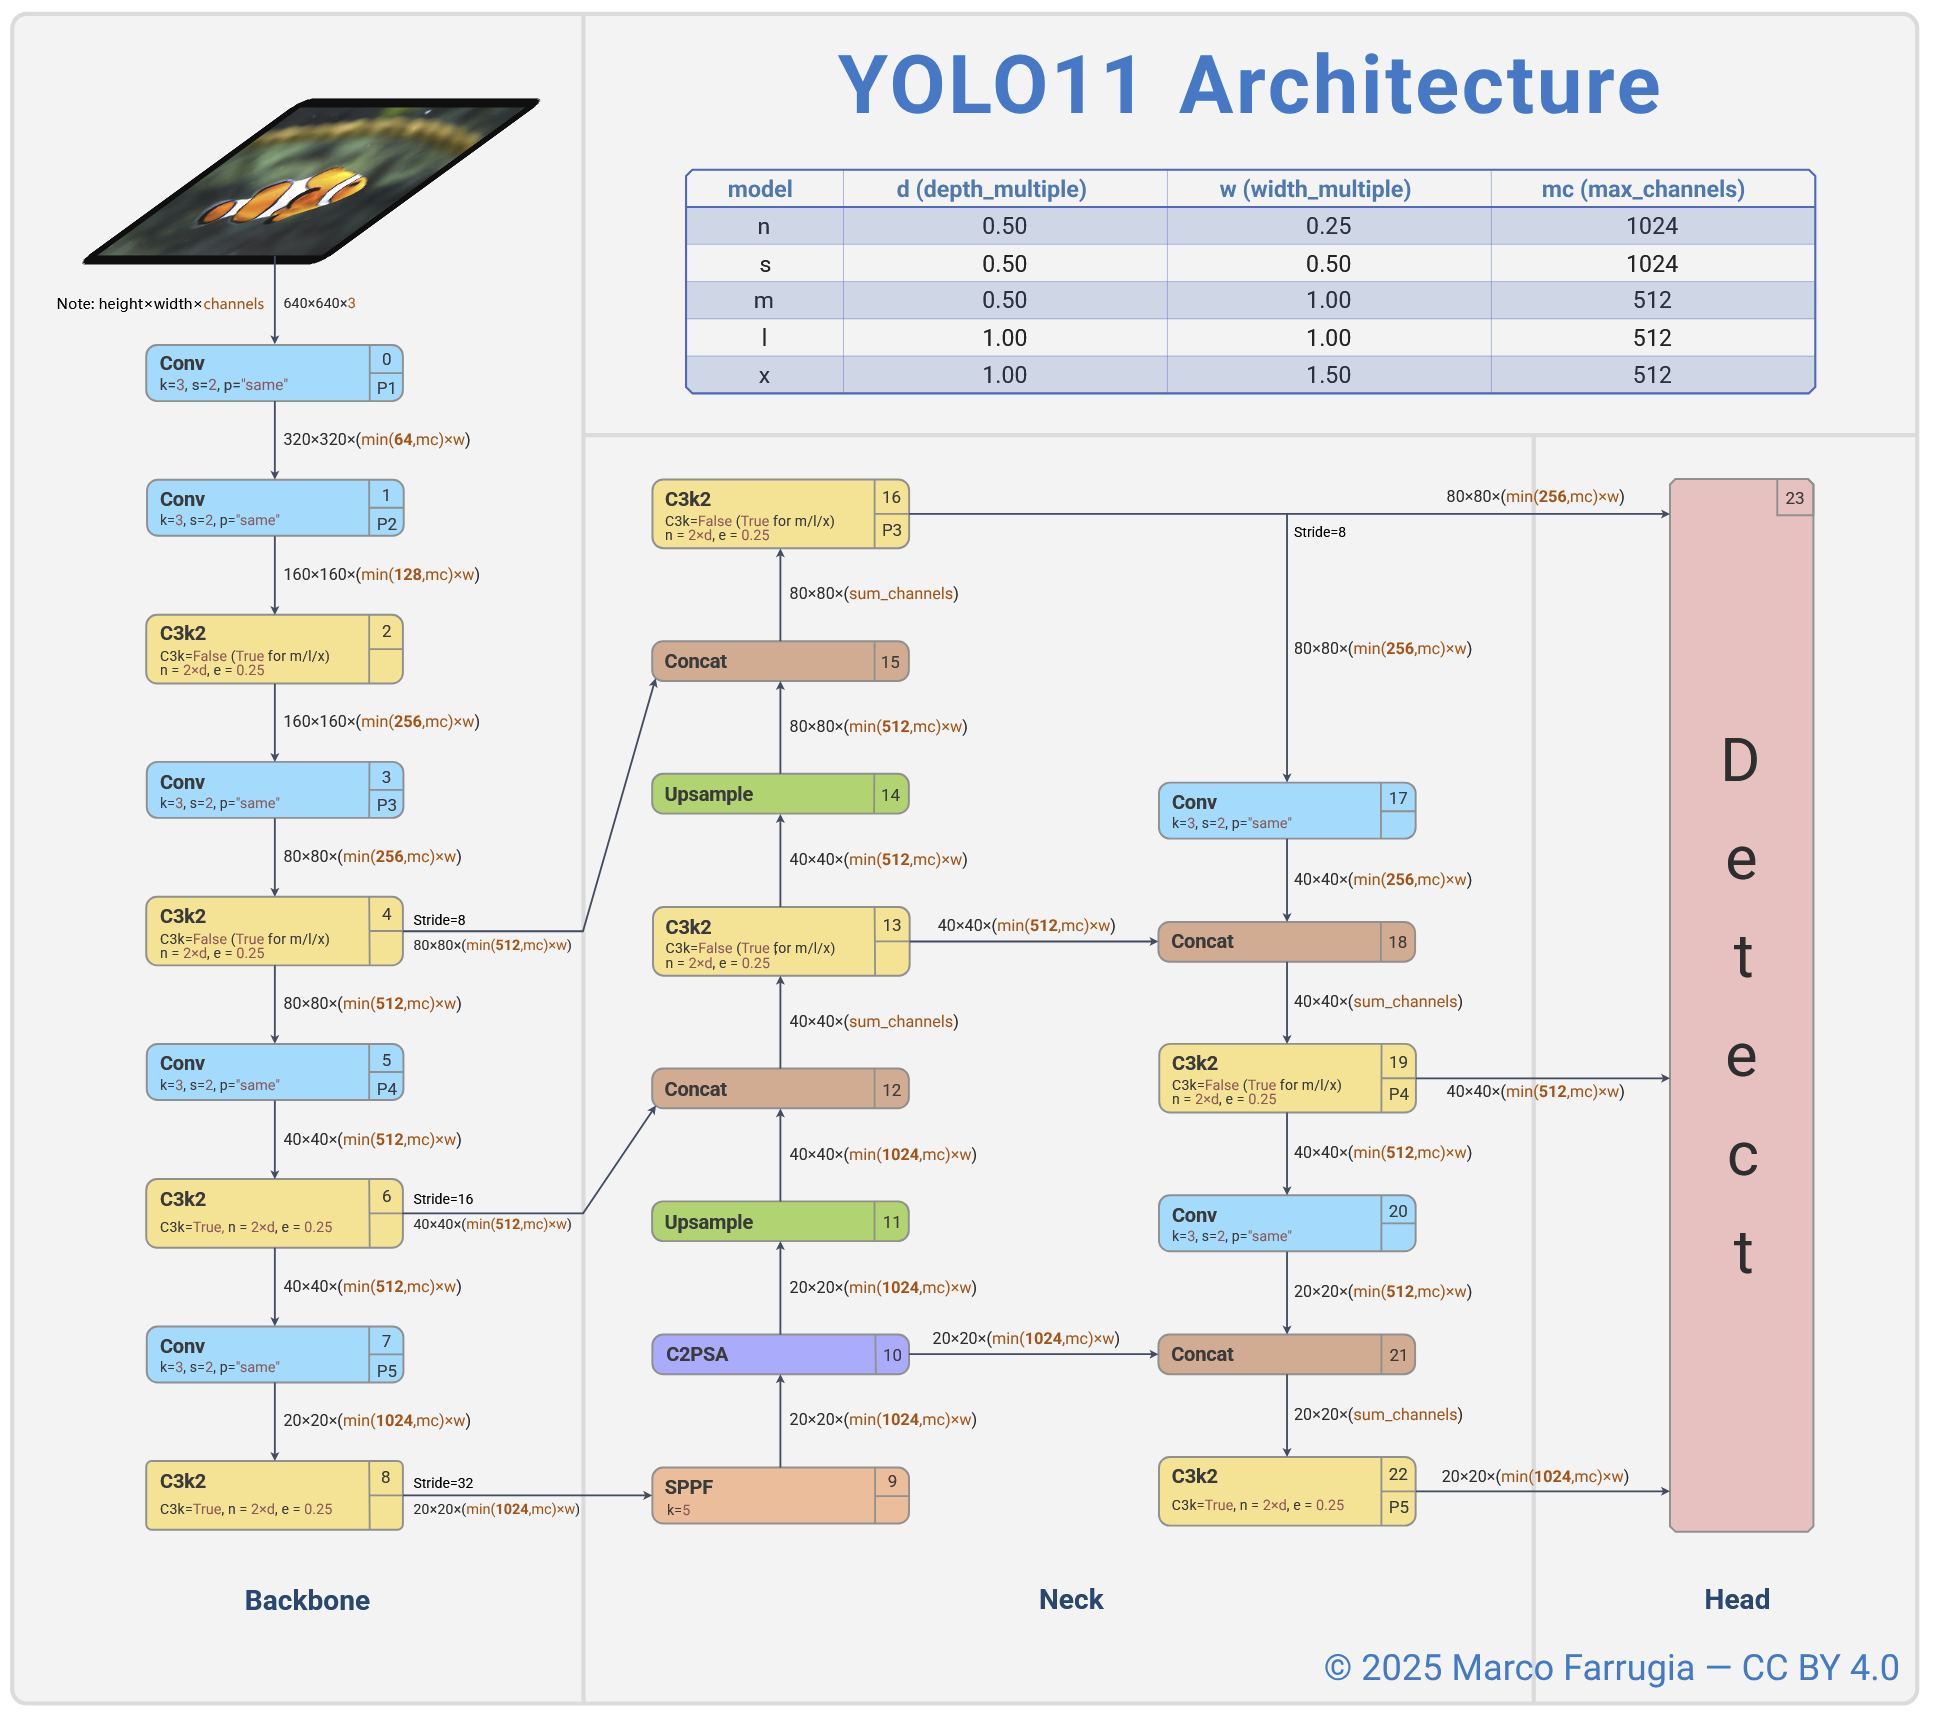
\includegraphics[width=0.95\textwidth]{figures/yolo11_architecture.png}
\caption{YOLO11 object-detection architecture used as the detector backend in this project. Source: Farrugia, CC BY 4.0, Zenodo DOI 10.5281/zenodo.17508018 \cite{farrugia2025yolo11diagram}.}
\label{fig:yolo11-architecture}
\end{figure}

\section{Temporal-Spatial Task Definition}
Frame-only parallelism is possible because frames are naturally ordered but mostly independent for this counting task. However, if only complete frames are distributed, the number of tasks may be too small to keep many MPI ranks busy, especially for short videos or small experiments. The project therefore uses a hybrid decomposition: each video is split by time into frames, and each frame is split by space into image tiles.

For a tile grid with \(R\) rows and \(C\) columns, frame \(F_i\) is decomposed into:
\begin{equation}
    F_i \rightarrow \{T_{i,1}, T_{i,2}, \ldots, T_{i,R \times C}\}.
\end{equation}
A parallel task is one YOLO inference on one frame-tile pair:
\begin{equation}
    task(i,j) = T_{i,j}, \qquad |\mathcal{T}| = N \times R \times C.
\end{equation}
This definition turns video inference into a task-parallel workload. Larger values of \(R\) and \(C\) create more tasks, which can improve utilization and load balancing. At the same time, finer tiling can reduce detector context, cut people near tile boundaries, create duplicate boxes, and increase the amount of data that must be gathered by rank 0. The problem is therefore not only to create more tasks, but also to choose a granularity that exposes parallelism without making merging and communication too expensive.

\section{Post-Processing Challenge}
The output of each tile is local to that tile. If a detected box has local coordinates \((x_1,y_1,x_2,y_2)\), these coordinates must be shifted back into the coordinate system of the original frame before the final count can be computed. For a tile whose top-left corner is \((x_s,y_s)\), the global coordinates are:
\begin{equation}
    x^{global} = x^{local} + x_s, \qquad
    y^{global} = y^{local} + y_s.
\end{equation}

This coordinate remapping is necessary but not sufficient. A person standing near a tile boundary may be detected in more than one tile. If all tile detections were counted directly, the final frame count could be too high. Therefore, rank 0 must merge detections from all tiles of the same frame, apply tile ownership filtering, and run global non-maximum suppression before producing the final count:
\begin{equation}
    B_i^{final} = NMS(B_i^{raw}, \theta), \qquad count(F_i)=|B_i^{final}|.
\end{equation}

This post-processing step is the main reason the problem is not purely embarrassingly parallel. Detector calls can be distributed across ranks, but final counting requires global information about all detections belonging to the same frame.

\section{Parallel-Programming Focus}
The central parallel-programming question is how to execute the frame-tile inference tasks across multiple MPI ranks while preserving the serial pipeline output and measuring the cost of distribution. The implementation uses task parallelism, static task mapping, centralized result gathering, and weighted process placement on a heterogeneous three-machine cluster.

The YOLO pipeline exercises the following parallel-programming concepts:
\begin{table}[H]
\centering
\caption{Parallel-programming concepts in the YOLO pipeline}
\label{tab:yolo-concepts}
\begin{tabularx}{\textwidth}{L{3.2cm} X}
\toprule
Concept & YOLO MPI implementation \\
\midrule
Parallelism level & Task parallelism across repeated YOLO inference calls \\
Decomposition & Hybrid temporal-spatial decomposition into frame-tile tasks \\
Mapping & 1D flattened task list with static block-cyclic ownership \\
Communication & Rank-local inference followed by centralized detection and metric gathering \\
Load balancing & Tile granularity and weighted process placement \\
Correctness target & MPI frame counts match serial frame counts after the same post-processing pipeline \\
\bottomrule
\end{tabularx}
\end{table}

\section{Correctness Targets}
The report uses two different notions of correctness. The first is parallel correctness. The serial YOLO baseline processes the same frame-tile task list without MPI distribution and applies the same post-processing pipeline. The MPI implementation is considered correct when it produces the same final people count as this serial baseline for each tested frame:
\begin{equation}
    \Delta_i = |count_{parallel}(F_i) - count_{serial}(F_i)|.
\end{equation}
The correctness experiment reports mismatched frames, maximum count error, and mean count error. A zero mismatch means the parallelization has preserved the serial pipeline output for the tested configuration.

The second notion is detector accuracy. Detector accuracy compares YOLO's predicted counts against human ground-truth counts from MOT17-derived data. This is a separate question because a model can undercount people in crowded frames even if the MPI implementation is perfectly consistent with the serial pipeline. The report therefore evaluates model accuracy and parallel correctness separately: one measures the quality of the detector, while the other measures whether the distributed implementation changes the pipeline result.

\chapter{Parallelization Methods}

\section{Task Parallel YOLO Inference}
The YOLO pipeline uses task-level parallelism over independent frame-tile inference tasks. The implementation is centered on \code{src/yolo\_mpi\_cpp.cpp} in the repository. Each MPI rank runs the same C++ program, and rank-local detector work is delegated to a long-lived Python YOLO worker.

\subsection{Temporal-Spatial Decomposition}
The input video is first decomposed by time into frames and then by space into image tiles. If the video has \(N\) frames and each frame is split into an \(R \times C\) grid, the total number of tasks is \(NRC\). Figure~\ref{fig:yolo-grid-split} compares the original frame with 2x2 and 5x4 tiling. The 2x2 grid keeps detector accuracy close to the original-frame baseline because it introduces fewer artificial tile borders, so fewer people are cut by tile edges before the final merge stage. Larger grids create more tasks and can improve scheduling flexibility, but they increase duplicate detections near tile borders and increase post-processing work.

\begin{figure}[!htbp]
\centering
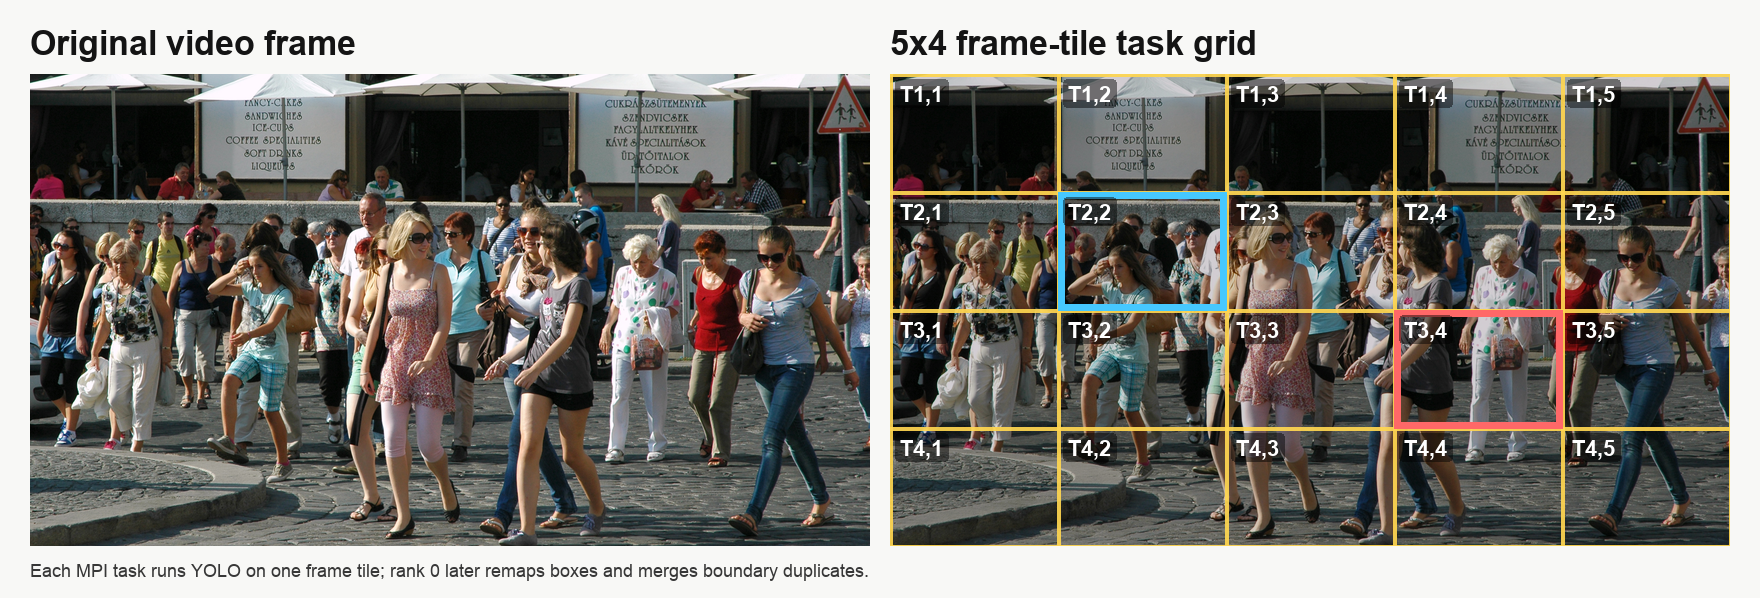
\includegraphics[width=0.98\textwidth]{figures/yolo_grid_split_visualization.png}
\caption{Hybrid temporal-spatial decomposition for YOLO video inference. The public-domain crowd frame is from Wikimedia Commons~\cite{keymeulen2011crowd}; the overlays show why coarse 2x2 tiling preserves accuracy better than finer 5x4 tiling while still creating independent frame-tile tasks.}
\label{fig:yolo-grid-split}
\end{figure}

\subsection{1D Mapping and Static Scheduling}
All frame-tile tasks are flattened into a one-dimensional list. For task index \(i\), chunk size \(k\), and \(P\) ranks, static block-cyclic scheduling assigns:
\begin{equation}
    owner(task_i) = \left\lfloor \frac{i}{k} \right\rfloor \bmod P.
\end{equation}
Static scheduling has low dispatch overhead because ranks can determine their own tasks locally. The measured repository results show that this advantage matters for the 600-frame 5x4 tiled YOLO workload.

\subsection{Communication and Merging}
After each rank finishes its assigned frame-tile tasks, it sends two types of data to rank 0: detected bounding boxes and timing metrics. The communication pattern is centralized. Worker ranks compute locally, then rank 0 gathers the local result payloads and performs the final merge.

For each detected person box, the worker stores:
\begin{equation}
    (frame\_id,\ tile\_id,\ x_1,\ y_1,\ x_2,\ y_2,\ score,\ class).
\end{equation}
The box coordinates are still relative to the local tile. Rank 0 first converts them back to original-frame coordinates:
\begin{equation}
    x^{global} = x^{local} + x_s,\qquad
    y^{global} = y^{local} + y_s,
\end{equation}
where \((x_s,y_s)\) is the top-left coordinate of the tile inside the original frame.

For each frame \(F_i\), rank 0 merges all detections from the \(R \times C\) tiles:
\begin{equation}
    B_i^{raw} = \bigcup_{j=1}^{RC} B_{i,j}.
\end{equation}
Since a person near a tile boundary may appear in more than one tile, duplicate boxes can occur. Rank 0 therefore applies tile-owner filtering followed by global non-maximum suppression:
\begin{equation}
    B_i^{final} = NMS(B_i^{raw}, \theta).
\end{equation}
The final people count for frame \(F_i\) is:
\begin{equation}
    count(F_i)=|B_i^{final}|.
\end{equation}
This centralized merge is necessary because each rank only sees its own assigned tiles, while duplicate removal requires all detections from the same frame.

\subsection{YOLO Algorithm Sketch}
\begin{algorithm}[H]
\caption{Static MPI YOLO people-counting pipeline}
\begin{algorithmic}[1]
\STATE Input video contains \(N\) frames; each frame is split into an \(R \times C\) grid.
\STATE Build task list \(\mathcal{T}\), where each task is \((frame\_id, tile\_id)\).
\STATE Flatten \(\mathcal{T}\) into a 1D list and assign task index \(q\) using
\[
    owner(q)=\left\lfloor \frac{q}{K} \right\rfloor \bmod P,
\]
where \(K\) is chunk size and \(P\) is the number of MPI ranks.
\FOR{each MPI rank \(r\) in parallel}
    \STATE Select all tasks whose owner is \(r\).
    \FOR{each selected task \((i,j)\)}
        \STATE Crop tile \(j\) from frame \(F_i\).
        \STATE Run YOLO inference on the tile.
        \STATE Keep only \code{person} detections.
        \STATE Store local boxes and timing metrics.
    \ENDFOR
\ENDFOR
\STATE Gather serialized detections and rank metrics to rank 0.
\IF{rank is 0}
    \FOR{each frame \(F_i\)}
        \STATE Convert tile-local boxes to global frame coordinates.
        \STATE Merge boxes from all tiles of frame \(F_i\).
        \STATE Apply tile-owner filtering and global NMS.
        \STATE Compute \(count(F_i)=|B_i^{final}|\).
    \ENDFOR
    \STATE Write per-frame counts and runtime metrics to CSV files.
\ENDIF
\end{algorithmic}
\end{algorithm}

\section{Parallel-Programming Focus}

\begin{table}[H]
\centering
\caption{Parallel-programming concepts in the YOLO MPI pipeline}
\label{tab:yolo-concepts}
\begin{tabularx}{\textwidth}{L{3.6cm} X}
\toprule
Concept & YOLO MPI implementation \\
\midrule

Parallelism level 
& Task-level parallelism: each task runs YOLO on one frame tile. \\

Decomposition 
& Hybrid temporal-spatial decomposition: video frames are divided into smaller image tiles. \\

Granularity
& Tile-level granularity: one task corresponds to one tile of one frame. \\

Mapping technique
& 1D task mapping: all frame-tile tasks are flattened into a list and assigned to MPI ranks using static block-cyclic distribution. \\

Communication strategy
& Each rank computes locally, then sends detections and timing results to rank 0 for merging. \\

Communication topology
& Master-worker topology: rank 0 gathers and post-processes results, while other ranks mainly perform inference. \\

Communication mode
& Blocking gather communication is used after local inference. \\

Load balancing
& Load balancing is considered through tile size, block-cyclic task assignment, and weighted process placement. \\

Correctness check
& The parallel output is correct if its frame-level people counts match the serial YOLO result after the same post-processing. \\

\bottomrule
\end{tabularx}
\end{table}

\chapter{Experimental Setup}

\section{Hardware and Cluster Environment}
The target environment is the macOS/OpenMPI cluster described by the repository hostfiles. GPU-oriented experiments use \code{configs/hosts\_macos\_gpu}; CPU/core-count experiments use \code{configs/hosts\_macos\_core} and weighted hostfiles when process counts exceed the three-rank GPU layout. Exact CPU, memory, process-slot, network, OpenMPI, and Python details must be taken from the final hardware evidence logs. They are intentionally not invented in this draft.

\begin{table}[H]
\centering
\caption{Hardware evidence to be filled from cluster logs}
\label{tab:hardware}
\begin{tabularx}{\textwidth}{L{2.4cm} L{2.2cm} L{2.6cm} L{2.0cm} X}
\toprule
Host & Role & CPU/SoC & Memory & Evidence source \\
\midrule
master & Pending log & Pending log & Pending log & final evidence logs \\
node1 & Pending log & Pending log & Pending log & final evidence logs \\
node2 & Pending log & Pending log & Pending log & final evidence logs \\
\bottomrule
\end{tabularx}
\end{table}

\section{Software Environment}
The implementation uses C++17, OpenMPI, a Python virtual environment, Ultralytics YOLO11n, and helper scripts under \path{scripts/runtime/}. The final report must record the actual OpenMPI version, Python version, YOLO package version, model path, detector device, and source video path from the run logs.

\section{Dataset and Input Size Definition}
The input size is the number of processed video frames \(N\). The input-size selection experiment runs several candidate frame counts and chooses an \(N\) whose wall-clock runtime is approximately 120--180 seconds on the target configuration. Speedup experiments then use \(2N\) frames to reduce startup noise.

\section{Metrics and Timing Methodology}
The report uses the CSV fields generated by the implementation:
\begin{itemize}
    \item \code{total\_ms\_with\_comm}: wall-clock runtime including MPI communication;
    \item \code{total\_ms\_without\_comm}: compute-oriented estimate excluding communication;
    \item \code{compute\_ms}, \code{yolo\_ms}, \code{comm\_ms}, \code{idle\_ms}: rank-level timing;
    \item \code{tasks\_done}: task count per rank;
    \item \code{correctness\_pass}: serial-versus-parallel verification status when \code{--verify 1}.
\end{itemize}
Speedup and efficiency are:
\begin{equation}
    S_p = \frac{T_1}{T_p}, \qquad E_p = \frac{S_p}{p}.
\end{equation}
Communication overhead is:
\begin{equation}
    \frac{T_{comm}}{T_{wall}}.
\end{equation}

\section{Required Experiment Matrix}
\begin{table}[H]
\centering
\caption{Required YOLO-only experiment matrix}
\label{tab:experiment-matrix}
\begin{tabularx}{\textwidth}{L{3.1cm} L{3.1cm} L{3.2cm} X}
\toprule
Experiment & Main setting & Required output & Report purpose \\
\midrule
Correctness & Static and dynamic, \code{--verify 1} & correctness CSVs & Verify parallel output against serial baseline. \\
Input size & Multiple \(N\), \(P=12\), dynamic & \code{raw/find\_N.csv} & Choose \(N\) near 120--180 s. \\
Granularity & Selected \(N\), one or more tile grids & \code{rank\_metrics.csv} & Per-rank task, compute, comm, idle analysis. \\
Scheduling & Same \(N,P\), static vs dynamic & scheduler CSV & Compare runtime and imbalance. \\
Speedup & \(2N\), \(P=1,2,4,8,12,24\) if possible & \code{raw/speedup.csv} & Compute \(S_p\) and \(E_p\). \\
Communication & Derived from summaries and rank metrics & communication CSV & Quantify \(T_{comm}/T_{wall}\). \\
\bottomrule
\end{tabularx}
\end{table}

\chapter{Results and Discussion}

No completed experiment CSV files were present in the inspected repository snapshot. This chapter is a results template for the final measured run package. It must be filled only from real CSV outputs; no runtime, speedup, correctness, hardware, or communication values are inferred.

\section{Correctness Verification}
Correctness is evaluated by running the implementation with \code{--verify 1}. The expected evidence is \code{summary.csv}, \code{frame\_counts.csv}, \code{bboxes.csv}, and \code{rank\_metrics.csv} for both static and dynamic scheduling.

\begin{table}[H]
\centering
\caption{Correctness verification table to be filled from measured CSV}
\label{tab:correctness}
\begin{tabularx}{\textwidth}{L{2.2cm} C{1.4cm} C{1.5cm} C{1.6cm} C{2.1cm} X}
\toprule
Schedule & Frames & Grid & Processes & Correctness pass & Evidence \\
\midrule
Static & Pending CSV & Pending CSV & Pending CSV & Pending CSV & static summary \\
Dynamic & Pending CSV & Pending CSV & Pending CSV & Pending CSV & dynamic summary \\
\bottomrule
\end{tabularx}
\end{table}

\section{Input Size Selection}
The input-size sweep chooses \(N\) so that wall-clock runtime is approximately 120--180 seconds on the selected cluster configuration.

\begin{table}[H]
\centering
\caption{Input size selection table to be filled from \code{find\_N.csv}}
\label{tab:input-size}
\begin{tabularx}{\textwidth}{C{1.3cm} C{1.4cm} C{1.5cm} C{2.5cm} C{2.7cm} X}
\toprule
\(N\) & Grid & \(P\) & Runtime with comm. & Runtime without comm. & Selection note \\
\midrule
Pending CSV & Pending & Pending & Pending CSV & Pending CSV & Pending CSV \\
\bottomrule
\end{tabularx}
\end{table}

\section{Granularity and Load Balance}
For each selected granularity case, the report will compute:
\begin{equation}
    G = \frac{N \times R \times C}{P}, \qquad
    imbalance = \frac{T_{max} - T_{min}}{T_{max}}.
\end{equation}

\begin{table}[H]
\centering
\caption{Per-rank granularity and load-balance table to be filled from \code{rank\_metrics.csv}}
\label{tab:granularity}
\begin{tabularx}{\textwidth}{C{1.0cm} C{1.6cm} C{1.8cm} C{1.9cm} C{1.8cm} C{1.7cm} X}
\toprule
Rank & Tasks & Compute ms & YOLO ms & Comm. ms & Idle ms & Host \\
\midrule
Pending & Pending CSV & Pending CSV & Pending CSV & Pending CSV & Pending CSV & Pending CSV \\
\bottomrule
\end{tabularx}
\end{table}

\section{Static vs Dynamic Scheduling}
Static and dynamic scheduling must be compared using the same \(N\), \(P\), tile grid, detector, model, and source video.

\begin{table}[H]
\centering
\caption{Static versus dynamic scheduling table to be filled from \code{scheduler\_comparison.csv}}
\label{tab:scheduler}
\begin{tabularx}{\textwidth}{L{1.8cm} C{1.2cm} C{1.4cm} C{2.3cm} C{2.3cm} C{1.8cm} X}
\toprule
Schedule & \(P\) & Grid & Runtime with comm. & Runtime without comm. & Imbalance & Note \\
\midrule
Static & Pending & Pending & Pending CSV & Pending CSV & Pending CSV & Pending CSV \\
Dynamic & Pending & Pending & Pending CSV & Pending CSV & Pending CSV & Pending CSV \\
\bottomrule
\end{tabularx}
\end{table}

\section{Speedup and Efficiency}
Speedup and efficiency are computed from the measured runtime:
\begin{equation}
    S_p = \frac{T_1}{T_p}, \qquad E_p = \frac{S_p}{p}.
\end{equation}
The final speedup experiment should use input size \(2N\). If \(P=24\) exceeds the intended physical-core configuration, it must be labeled as oversubscription.

\begin{table}[H]
\centering
\caption{Speedup table to be filled from \code{speedup.csv}}
\label{tab:speedup}
\begin{tabularx}{\textwidth}{C{1.0cm} C{2.1cm} C{2.2cm} C{1.9cm} C{1.9cm} X}
\toprule
\(P\) & Runtime with comm. & Runtime without comm. & \(S_p\) & \(E_p\) & Note \\
\midrule
Pending & Pending CSV & Pending CSV & Pending CSV & Pending CSV & Pending CSV \\
\bottomrule
\end{tabularx}
\end{table}

\section{Communication Overhead}
Communication overhead is:
\begin{equation}
    \frac{T_{comm}}{T_{wall}}.
\end{equation}
The numerator must come from \code{comm\_ms\_total} or aggregated \code{rank\_metrics.csv}; the denominator must come from \code{total\_ms\_with\_comm}.

\begin{table}[H]
\centering
\caption{Communication overhead table to be filled from measured summaries}
\label{tab:communication}
\begin{tabularx}{\textwidth}{L{2.2cm} C{1.1cm} C{2.2cm} C{2.0cm} C{2.0cm} X}
\toprule
Run & \(P\) & \(T_{wall}\) & \(T_{comm}\) & Ratio & Evidence \\
\midrule
Pending CSV & Pending & Pending CSV & Pending CSV & Pending CSV & communication summary \\
\bottomrule
\end{tabularx}
\end{table}

\section{Bottleneck Analysis}
The final bottleneck analysis should be evidence-driven. Possible causes include task imbalance, heterogeneous host speeds, repeated tile-border work, communication overhead from dynamic scheduling, and Apple MPS contention when multiple ranks share accelerator resources. This draft does not rank those causes because the required CSV evidence has not yet been collected.

\chapter{Conclusion}

This report presents the implemented YOLO-MPI people-counting system as a parallel inference runtime. The method decomposes a video into frame-tile tasks, supports static block-cyclic scheduling and dynamic master-worker scheduling, uses rank-local YOLO workers, and aggregates final detections on rank 0 with duplicate removal and NMS.

The implementation evidence supports a YOLO-only report. A second VGG16, convolution, or halo-exchange method is not implemented and is therefore not included. The communication design is also reported conservatively: payload transfer uses blocking MPI calls, while \code{MPI\_Iprobe} is used only for polling in the dynamic scheduler.

The remaining work before final submission is experimental rather than methodological. The final PDF should replace all pending result placeholders with measured CSV evidence for correctness, input size selection, granularity, scheduling, speedup, and communication overhead.

\chapter{Member Contributions}

Table~\ref{tab:contributions} records the responsibility split based on the current repository contents.

\begin{table}[H]
\centering
\caption{Draft member contributions}
\label{tab:contributions}
\begin{tabularx}{\textwidth}{L{4.2cm} L{2.8cm} X}
\toprule
Member & Student ID & Contribution \\
\midrule
Luu Hieu An & 202400093 & Report integration, repository evidence audit, final presentation alignment, and result table preparation. \\
Nguyen Phu An & 20235466 & Cluster setup, OpenMPI execution, hardware evidence collection, and hostfile/placement experiments. \\
Pham Chi Bang & 20235477 & C++/MPI implementation, YOLO scheduling pipeline, and result aggregation support. \\
Nguyen Thanh Lam & 20235518 & Plot generation, speedup table preparation, experimental discussion, and final report polishing. \\
\bottomrule
\end{tabularx}
\end{table}


\clearpage
\bibliographystyle{plain}
\bibliography{references}

\end{document}
